\documentclass[italian]{article}
\usepackage[T1]{fontenc}
\usepackage[utf8]{inputenc}
\usepackage{lmodern}
\usepackage{hyperref}
\usepackage[a4paper,top=3cm,bottom=3cm,left=2.5cm,right=2.5cm]{geometry}
\usepackage[italian]{babel}
\usepackage{listings} %Per inserire codice
\usepackage[usenames]{color} %Per permettere la colorazione dei caratteri 
%Define the listing package
\usepackage{listings} %code highlighter
\usepackage{color} %use color
\usepackage{graphicx}
\graphicspath{ {./images/} }
\definecolor{mygreen}{rgb}{0,0.6,0}
\definecolor{mygray}{rgb}{0.5,0.5,0.5}
\definecolor{mymauve}{rgb}{0.58,0,0.82}

%Customize a bit the look
\lstset{ %
	backgroundcolor=\color{white}, % choose the background color; you must add \usepackage{color} or \usepackage{xcolor}
	basicstyle=\footnotesize, % the size of the fonts that are used for the code
	breakatwhitespace=false, % sets if automatic breaks should only happen at whitespace
	breaklines=true, % sets automatic line breaking
	captionpos=b, % sets the caption-position to bottom
	commentstyle=\color{mygreen}, % comment style
	deletekeywords={...}, % if you want to delete keywords from the given language
	escapeinside={\%*}{*)}, % if you want to add LaTeX within your code
	extendedchars=true, % lets you use non-ASCII characters; for 8-bits encodings only, does not work with UTF-8
	frame=single, % adds a frame around the code
	keepspaces=true, % keeps spaces in text, useful for keeping indentation of code (possibly needs columns=flexible)
	keywordstyle=\color{blue}, % keyword style
	% language=Octave, % the language of the code
	morekeywords={*,...}, % if you want to add more keywords to the set
	numbers=left, % where to put the line-numbers; possible values are (none, left, right)
	numbersep=5pt, % how far the line-numbers are from the code
	numberstyle=\tiny\color{mygray}, % the style that is used for the line-numbers
	rulecolor=\color{black}, % if not set, the frame-color may be changed on line-breaks within not-black text (e.g. comments (green here))
	showspaces=false, % show spaces everywhere adding particular underscores; it overrides 'showstringspaces'
	showstringspaces=false, % underline spaces within strings only
	showtabs=false, % show tabs within strings adding particular underscores
	stepnumber=1, % the step between two line-numbers. If it's 1, each line will be numbered
	stringstyle=\color{mymauve}, % string literal style
	tabsize=2, % sets default tabsize to 2 spaces
	title=\lstname % show the filename of files included with \lstinputlisting; also try caption instead of title
}
%END of listing package%

\definecolor{darkgray}{rgb}{.4,.4,.4}
\definecolor{purple}{rgb}{0.65, 0.12, 0.82}

%define Javascript language
\lstdefinelanguage{JavaScript}{
	keywords={typeof, new, true, false, catch, function, return, null, catch, switch, var, if, in, while, do, else, case, break},
	keywordstyle=\color{blue}\bfseries,
	ndkeywords={class, export, boolean, throw, implements, import, this},
	ndkeywordstyle=\color{darkgray}\bfseries,
	identifierstyle=\color{black},
	sensitive=false,
	comment=[l]{//},
	morecomment=[s]{/*}{*/},
	commentstyle=\color{purple}\ttfamily,
	stringstyle=\color{red}\ttfamily,
	morestring=[b]',
	morestring=[b]"
}

\lstset{
	language=JavaScript,
	extendedchars=true,
	basicstyle=\footnotesize\ttfamily,
	showstringspaces=false,
	showspaces=false,
	numbers=left,
	numberstyle=\footnotesize,
	numbersep=9pt,
	tabsize=2,
	breaklines=true,
	showtabs=false,
	captionpos=b
}
\author{
	Daniele Rigon - 857319 \\
}


\begin{document}
	
	\title{Tesi - Geolocation API}
	\maketitle
	
	\tableofcontents
	\pagebreak
	
	
	\section{Overview geolocation}
	Per quanto riguarda le Geolocation Api, su un dispositivo mobile avremo un set di coordinate provenienti dal sensore GPS, mentre su un portatile potremo usare il posizionamento legato all’ip della connessione internet.
	Le API per la geolocalizzazione permettono agli utenti di fornire la propria posizione alle applicazioni web. Per proteggere la privacy all'utente viene richiesta l'autorizzazione all'uso della posizione.
	
	\section{Specifiche}
	Esistono praticamente solo due metodi a disposizione, getCurrentPosition e watchPosition (+ clearWatch), entrambi utili a ottenere la posizione corrente. 
	La differenza tra i due va ricercata nella loro periodicità, mentre il primo metodo fornisce il dato una sola volta, il secondo si attiva automaticamente ogniqualvolta la posizione cambi, o ogni tot intervallo di tempo.
	La sintassi per invocare questi metodi è la seguente:
	\begin{lstlisting}[language=JavaScript]
	navigator.geolocation.getCurrentPosition(inCasoDiSuccesso, opzInCasoDiErrore, opzioni); 
	navigator.geolocation.watchPosition(inCasoDiSuccesso, opzInCasoDiErrore, opzioni);
	\end{lstlisting}

	\subsection{Oggetto della geolocalizzazione}
	Le API di geolocalizzazione sono pubblicate tramite l'oggetto navigator.geolocation. Se l'oggetto esiste, il servizio di geolocalizzazione è disponibile. Per testare l'esistenza di tale oggetto:
	\begin{lstlisting}[language=JavaScript]
		if ("geolocation" in navigator) {
		/* la geolocalizzazione e disponibile */
		} else {
		/* la geolocalizzazione NON e disponibile */
		}
	\end{lstlisting}
	
	\subsection{Metodi}
	\subsubsection{GetCurrentPosition}
	\begin{lstlisting}[language=JavaScript]
	navigator.geolocation.getCurrentPosition(function(position) {
		do_something(position.coords.latitude,position.coords.longitude);
	});
	\end{lstlisting}
	\begin{flushleft}
		L'esempio qui sopra chiama la funzione dosomething() quando la posizione viene calcolata.
		!=
		La funzione invocata in caso di successo con tutte le info:
	\end{flushleft}
\pagebreak
	\begin{lstlisting}
	inCasoDiSuccesso = function(position){ 
	alert( "Posizione delle: " + position.timestamp.getHours() + ":" +
	position.timestamp.getMinutes() + "n" + 
	"Accuratezza delle coordinate: " + position.coords.accuracy + " mt; n" + 
	"Latitudine: " + position.coords.latitude + " gradi; n" + 
	"Longitudine: " + position.coords.longitude + "gradi; n" + 
	"Accuratezza dell'altezza: " + position.coords.altitudeAccuracy + " mt; n" + 
	"Altezza: " + position.coords.altitude + " mt; n" + 
	"Direzione: " + position.coords.heading + " gradin " +
	"(0 = Nord, 90 = Ovest, 180 = Sud, 270 = Est);n" + 
	"Velocita: " + position.coords.speed + " m/s;"
	);
	}
	\end{lstlisting}
	\begin{flushleft}
		Nel frammento di codice appena illustrato possiamo vedere tutte le informazioni estraibili dalla struttura Position. Chiaramente, a seconda del device sul quale viene effettuata l’interrogazione, non tutte saranno sempre disponibili, in tal caso il loro valore sarà impostato a null. 
	\end{flushleft}
	\begin{figure}[h]
		\centering
		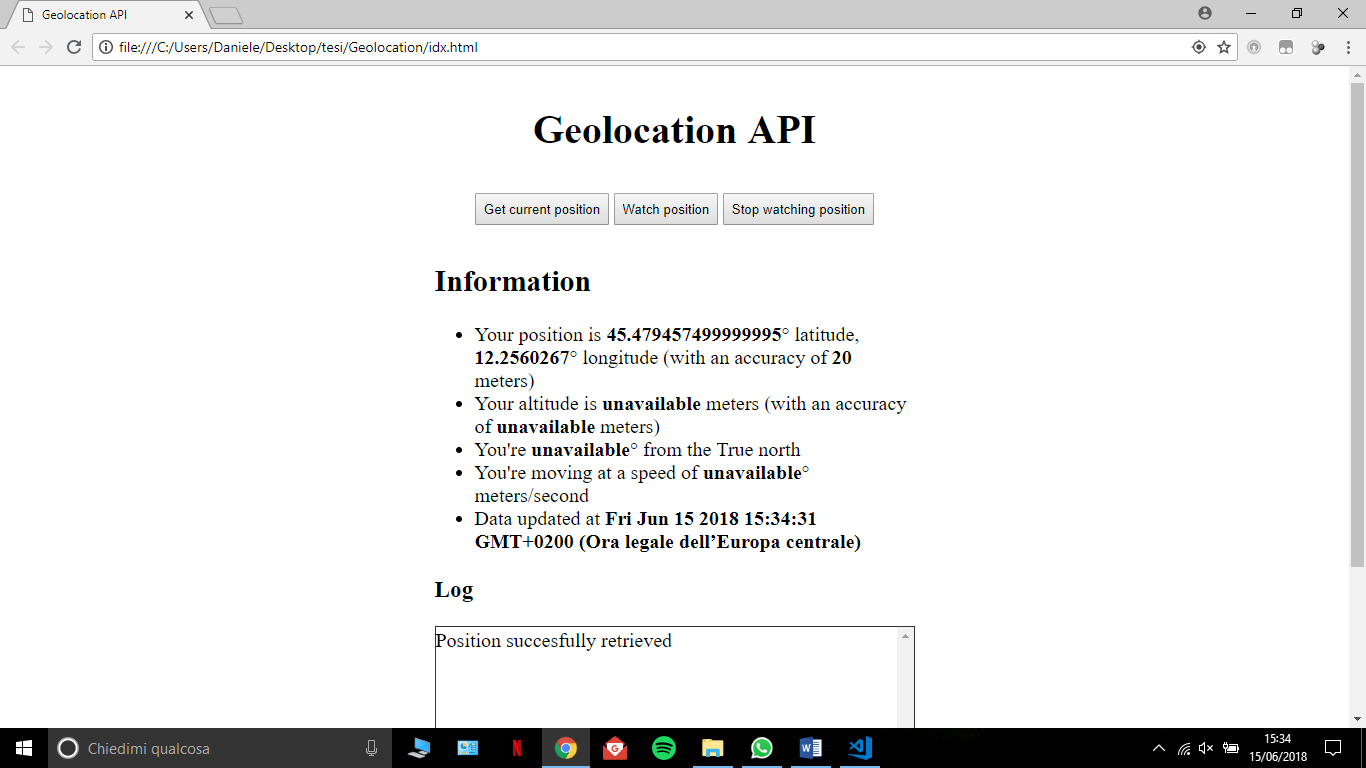
\includegraphics[width=1\linewidth]{img}
		\caption[Prova]{Prova info Geolocation.}
		\label{fig:Info Geolocation}
	\end{figure}
	\begin{flushleft}
		In caso invece si verifichi un errore la funzione preposta deve accettare anch’essa un parametro, un oggetto di tipo PositionError  contenente un codice di errore ed un messaggio ad uso di debug, ad esempio:
	\end{flushleft}
	\begin{lstlisting}
		message.opzInCasoDiErrore = function(error){ 
		alert( "Errore " + error.code + ": " + error.message);
		}
	\end{lstlisting}

	\subsubsection{WatchPosition}
	Se la posizione cambia (perché il dispositivo si sposta o perché viene calcolata una posizione più accurata), si può settare una funzione che viene chiamata quando la posizione attuale si aggiorna. Basta usare la funzione watchPosition(), che ha gli stessi parametri di input di getCurrentPosition(). Questa funzione viene chiamata più volte così da permettere al browser di sapere sempre la posizione del dispositivo. La funzione di errore è opzionale come lo era per getCurrentPosition().
	
	\begin{lstlisting}
	var watchID = navigator.geolocation.watchPosition(function(position) {
		do_something(position.coords.latitude, position.coords.longitude);
	});
	\end{lstlisting}
	\begin{flushleft}
	Il metodo watchPosition() ritorna un ID numerico che può essere usato per identificare univocamente il controllo della posizione; 
	Nota: si può usare questo valore insieme al metodo clearWatch() per fermare il controllo della posizione.
	\end{flushleft}
	\begin{lstlisting}
	navigator.geolocation.clearWatch(watchID);
	\end{lstlisting}
	\begin{flushleft}
	Infatti, un'invocazione del metodo watchPosition può essere successivamente interrotta utilizzando la funzione clearWatch, 
	come nell’esempio seguente:
	\end{flushleft}
	\begin{lstlisting}
	<!doctype html> 
	<html> 
	<head>
	<title> Un esempio di watchPosition</title> 
	<script> 
	var id_watch = null;
	
	inCasoDiSuccesso = function(position){ 
		document.getElementById("posizione_corrente").insertAdjacentHTML('beforeend',
		"<li> Lat: " + position.coords.latitude + ", Lon: " + position.coords.longitude + );
		"</li>"
		);
	}
	
	sospendiLaRicezione = function(){ 
		navigator.geolocation.clearWatch(id_watch);
	}
	
	window.onload = function(){ 
		id_watch = navigator.geolocation.watchPosition(inCasoDiSuccesso);
	}
	</script> 
	</head>
	<body> 
	<h1>La tua posizione attuale</h1> 
	<menu type="toolbar">
	<button type="button" onclick="sospendiLaRicezione()"> 
	sospendi la ricezione di dati geospaziali
	</button> 
	</menu>
	<ul id="posizione_corrente">
	</ul> 
	</body>
	</html>
	\end{lstlisting}
	
	\subsubsection{ClearPosition}
	
	\subsection{Supporto compatibilità web}
	\begin{figure}[h]
		\centering
		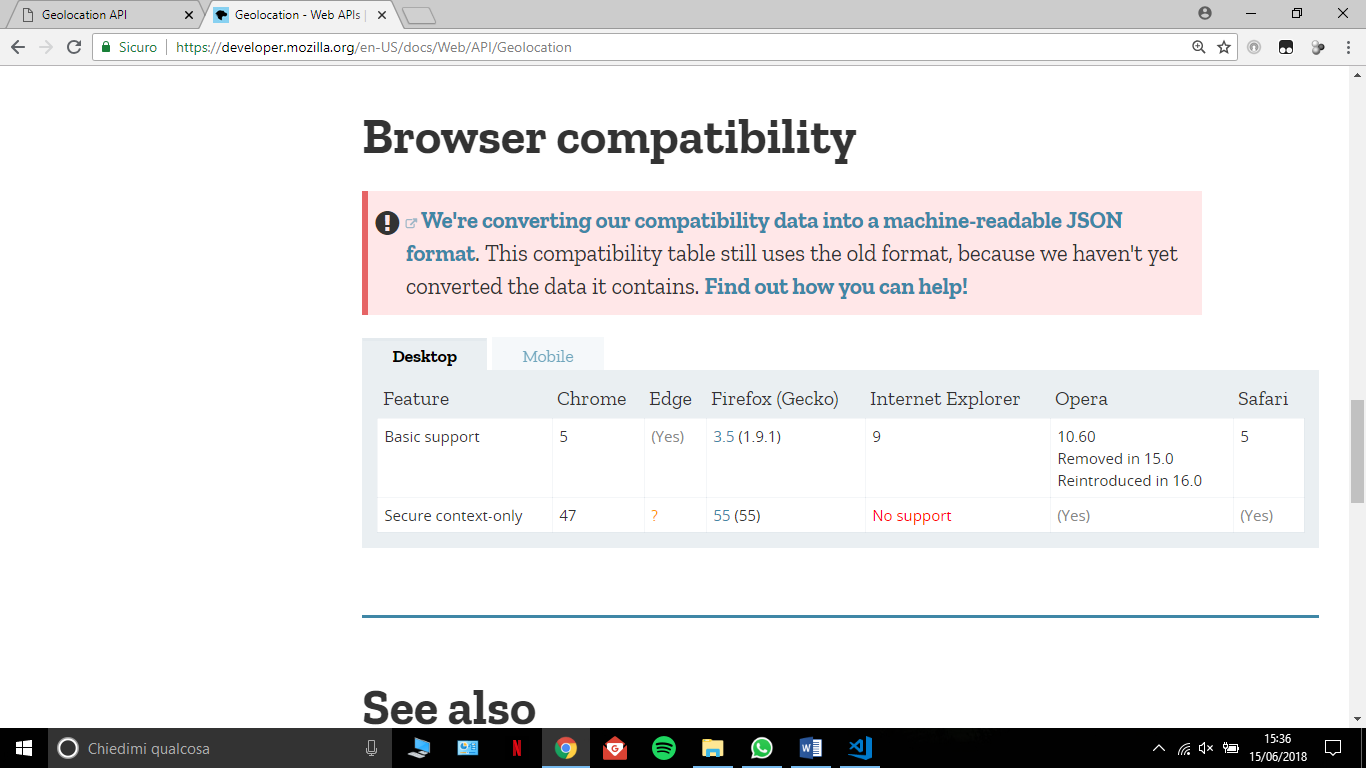
\includegraphics[width=1\linewidth]{web1}
		\caption[Prova]{Browser compatibility}
		\label{fig:Browser compatibility}
	\end{figure}
	
	\subsection{Problemi sicurezza/privacy}
	\url{https://developers.google.com/web/updates/2016/04/geolocation-on-secure-contexts-only}
	
	\subsection{Come la geolocation api trova la posizione esatta}
	\url{https://stackoverflow.com/questions/4213410/how-does-html5-geolocation-work}
	
	\subsection{Test Result}
	\url{https://wpt.fyi/results/geolocation-API}
	
	\subsection{Test Repository}
	\url{https://github.com/web-platform-tests/wpt/tree/master/geolocation-API}
	
\end{document}